\documentclass[
12pt, % Main document font size
a4paper, % Paper type, use 'letterpaper' for US Letter paper
%oneside, % One page layout (no page indentation)
twoside, % Two page layout (page indentation for binding and different headers)
headinclude,footinclude, % Extra spacing for the header and footer
BCOR5mm, % Binding correction
]{scrartcl}

% Change the name of the report here.
\def\ArticleTitle{ {{-cookiecutter.title-}} }

% This file specifies the document structure and layout
%%%%%%%%%%%%%%%%%%%%%%%%%%%%%%%%%%%%%%%%%
% Arsclassica Article
% Structure Specification File
%
% This file has been downloaded from:
% http://www.LaTeXTemplates.com
%
% Original author:
% Lorenzo Pantieri (http://www.lorenzopantieri.net) with extensive modifications by:
% Vel (vel@latextemplates.com)
%
% License:
% CC BY-NC-SA 3.0 (http://creativecommons.org/licenses/by-nc-sa/3.0/)
%
%%%%%%%%%%%%%%%%%%%%%%%%%%%%%%%%%%%%%%%%%

%----------------------------------------------------------------------------------------
%	REQUIRED PACKAGES
%----------------------------------------------------------------------------------------


\usepackage[
nochapters, % Turn off chapters since this is an article
beramono, % Use the Bera Mono font for monospaced text (\texttt)
eulermath,% Use the Euler font for mathematics
pdfspacing, % Makes use of pdftex’ letter spacing capabilities via the microtype package
dottedtoc % Dotted lines leading to the page numbers in the table of contents
]{classicthesis} % The layout is based on the Classic Thesis style

\usepackage{arsclassica} % Modifies the Classic Thesis package

\usepackage[T1]{fontenc} % Use 8-bit encoding that has 256 glyphs

\usepackage[utf8]{inputenc} % Required for including letters with accents

% Bibliography package (avoid printing location and specific date information.
\usepackage[
  backend=biber,
  abbreviate=true,
  firstinits=true,
  isbn=false,
  url=false,
  doi=false,
  eprint=false
]{biblatex}
\renewbibmacro{in:}{}
\AtEveryBibitem{%
        \clearfield{day}%
        \clearfield{month}%
        \clearfield{endday}%
        \clearfield{endmonth}%
        \clearlist{location}%
        \clearlist{address}%
        \clearfield{titleaddon}%
        \clearfield{pages}%
        \clearfield{language}%
        \clearlist{editor}%
        \clearfield{series}%
        \clearfield{booktitle}%
}

%
% Control display of captions
% You could change the names below to Fig., Tab. for shorter versions.
\usepackage[font=footnotesize,labelfont=bf,tableposition=bottom,figurename=Figure,tablename=Table]{caption}
\newenvironment{captiontext}{%
   \begin{center}%
     \begin{minipage}{0.9\linewidth}%
       \renewcommand{\baselinestretch}{0.8}%
         \footnotesize}%
   {\renewcommand{\baselinestretch}{1.0}%
      \end{minipage}%
        \end{center}}
\captionsetup[table]{singlelinecheck=off}

% For including math equations, theorems, symbols, etc
\usepackage{amsmath,amssymb,amsthm}

\usepackage{comment}
\usepackage{endnotes}
\usepackage{todonotes}
\makeatletter
\renewcommand*\makeenmark{\hbox{\textsuperscript{\@Alph{\theenmark}}}}
\makeatother

\usepackage{graphicx} % Required for including images
\graphicspath{{Figures/}  } % Set the default folder for images, observe the double curly brackets.

\usepackage{enumitem} % Required for manipulating the whitespace between and within lists

\usepackage{lipsum} % Used for inserting dummy 'Lorem ipsum' text into the template

\usepackage{subfig} % Required for creating figures with multiple parts (subfigures)

\usepackage{varioref} % More descriptive referencing

% Control list of authors and their affiliations
\usepackage[auth-sc]{authblk}
\renewcommand\Affilfont{\itshape\small}

\usepackage{xargs}

\usepackage{siunitx}
\usepackage{xspace}
\usepackage[all]{foreign}

\usepackage[boxed,noline]{algorithm2e}
\usepackage{tikz}
\usetikzlibrary{trees}

%----------------------------------------------------------------------------------------
%	THEOREM STYLES
%---------------------------------------------------------------------------------------

\theoremstyle{definition} % Define theorem styles here based on the definition style (used for definitions and examples)
\newtheorem{definition}{Definition}

\theoremstyle{plain} % Define theorem styles here based on the plain style (used for theorems, lemmas, propositions)
\newtheorem{theorem}{Theorem}
\newtheorem{axiom}[theorem]{Axiom}
\newtheorem{case}[theorem]{Case}
\newtheorem{conclusion}[theorem]{Conclusion}
\newtheorem{condition}[theorem]{Condition}
\newtheorem{conjecture}[theorem]{Conjecture}
\newtheorem{corollary}[theorem]{Corollary}
\newtheorem{criterion}[theorem]{Criterion}
\newtheorem{example}[theorem]{Example}
\newtheorem{exercise}[theorem]{Exercise}
\newtheorem{lemma}[theorem]{Lemma}
\newtheorem{notation}[theorem]{Notation}
\newtheorem{problem}[theorem]{Problem}
\newtheorem{proposition}[theorem]{Proposition}
\newtheorem{remark}[theorem]{Remark}
\newtheorem{solution}[theorem]{Solution}
\newtheorem{summary}[theorem]{Summary}

\theoremstyle{remark} % Define theorem styles here based on the remark style (used for remarks and notes)
\newtheorem{acknowledgement}[theorem]{Acknowledgement}

%----------------------------------------------------------------------------------------
%	HYPERLINKS
%---------------------------------------------------------------------------------------

\hypersetup{
%draft, % Uncomment to remove all links (useful for printing in black and white)
colorlinks=true, breaklinks=true, bookmarks=true,bookmarksnumbered,
urlcolor=webbrown, linkcolor=RoyalBlue, citecolor=webgreen, % Link colors
pdftitle={\ArticleTitle}, % PDF title
pdfauthor={\textcopyright}, % PDF Author
pdfsubject={}, % PDF Subject
pdfkeywords={}, % PDF Keywords
pdfcreator={pdfLaTeX}, % PDF Creator
pdfproducer={LaTeX with hyperref and ClassicThesis} % PDF producer
}

\def\sectionautorefname{Sec.}
\def\subsectionautorefname{Sec.}
\def\subsubsectionautorefname{Sec.}
\def\figureautorefname{Fig.}
\def\subfigureautorefname{Fig.}

\newcommand{\vautoref}[1]{\sectionautorefname~\vref{#1}\xspace}



%----------------------------------------------------------------------------------------
%	TITLE AND AUTHOR(S)
%----------------------------------------------------------------------------------------

\title{\normalfont\spacedallcaps{\ArticleTitle}} % The article title

%\subtitle{Subtitle} % Uncomment to display a subtitle

 % The article author(s) - author affiliations need to be specified in the AUTHOR AFFILIATIONS block
\author{\spacedlowsmallcaps{John Smith* \& James Smith\textsuperscript{1}}}

% An optional date to appear under the author(s)
\date{}

%----------------------------------------------------------------------------------------

\bibliography{ {{-cookiecutter.bib_file_name-}} }


% Specify custom hyphenation points in words with dashes where you
% would like hyphenation to occur, or alternatively, don't put any
% dashes in a word to stop hyphenation altogether
\hyphenation{hy-phen-ation}

% It is a good idea to create macros for commonly used terms
\def\Internet{\emph{Internet}\xspace}
\def\WWW{\emph{WWW}\xspace}

% Specify custom commands here
\newcommand{\TODO}[2]{\textcolor{red}{#1}\todo{#2}\xspace}
\newcommand{\todoref}[1]{\textcolor{red}{Section XX}\todo{#1}\xspace}
\newcommandx{\change}[2][1=]{\todo[linecolor=blue,backgroundcolor=blue!25,bordercolor=blue,#1]{#2}}


%%% Local Variables:
%%% mode: latex
%%% TeX-master: "{{cookiecutter.file_name}}"
%%% End:



\begin{document}


%----------------------------------------------------------------------------------------
%	HEADERS
%----------------------------------------------------------------------------------------

% The header for all pages (oneside) or for even pages (twoside)
\renewcommand{\sectionmark}[1]{\markright{\spacedlowsmallcaps{#1}}}
% Uncomment the following when using the twoside option - this modifies the header on odd pages
\renewcommand{\subsectionmark}[1]{\markright{\thesubsection~#1}}

 % The header style
\lehead{\mbox{\llap{\small\thepage\kern1em\color{halfgray} \vline}\color{halfgray}\hspace{0.5em}\rightmark\hfil}}

\pagestyle{scrheadings} % Enable the headers specified in this block

%----------------------------------------------------------------------------------------
%	TABLE OF CONTENTS & LISTS OF FIGURES AND TABLES
%----------------------------------------------------------------------------------------

\maketitle % Print the title/author/date block

\setcounter{tocdepth}{2} % Set the depth of the table of contents to show sections and subsections only

\tableofcontents % Print the table of contents

\listoffigures % Print the list of figures

\listoftables % Print the list of tables

%----------------------------------------------------------------------------------------
%	ABSTRACT
%----------------------------------------------------------------------------------------

\section*{Abstract} % This section will not appear in the table of contents due to the star (\section*)

\lettrineabstract{%
  Lorem ipsum dolor sit amet, consectetur adipiscing elit. Fusce
  maximus nisi ligula. Morbi laoreet ex ligula, vitae lobortis purus
  mattis vel. Vestibulum ante ipsum primis in faucibus orci luctus et
  ultrices posuere cubilia Curae; Donec ac metus ut turpis mollis
  placerat et nec enim. Duis tristique nibh maximus faucibus
  facilisis. Praesent in consequat leo. Maecenas condimentum ex
  rhoncus, elementum diam vel, malesuada ante.%
}

\lipsum[1] % Dummy text

%----------------------------------------------------------------------------------------
%	AUTHOR AFFILIATIONS
%----------------------------------------------------------------------------------------

\let\thefootnote\relax\footnotetext{* \textit{Department of Biology, University of Examples, London, United Kingdom}}

\let\thefootnote\relax\footnotetext{\textsuperscript{1} \textit{Department of Chemistry, University of Examples, London, United Kingdom}}

%----------------------------------------------------------------------------------------

\newpage % Start the article content on the second page, remove this if you have a longer abstract that goes onto the second page

\section{Introduction}
\label{sec:introduction}

\section{Introduction}%
\label{sec:introduction}

This sentence requires citation \autocite{Reference1}. %
This sentence requires multiple citations to imply that it is better
supported \autocite{Reference2,Reference3}. %
Finally, when conducting an appeal to authority, it can be useful to
cite a reference in-text, much like \autocite{Reference1} do quite a
bit. %
Oh, and make sure to check out the bear in \autoref{bear}.

\Blindtext

\begin{align}
        A =
        \begin{bmatrix}
                A_{11} & A_{21} \\
                A_{21} & A_{22}
        \end{bmatrix}
\end{align}

\subsection{Subsection}

Nam ante risus, tempor nec lacus ac, congue pretium dui. Donec a nisl est. Integer accumsan mauris eu ex venenatis mollis. Aliquam sit amet ipsum laoreet, mollis sem sit amet, pellentesque quam. Aenean auctor diam eget erat venenatis laoreet. In ipsum felis, tristique eu efficitur at, maximus ac urna. Aenean pulvinar eu lorem eget suscipit. Aliquam et lorem erat. Nam fringilla ante risus, eget convallis nunc pellentesque non. Donec ipsum nisl, consectetur in magna eu, hendrerit pulvinar orci. Mauris porta convallis neque, non viverra urna pulvinar ac. Cras non condimentum lectus. Aliquam odio leo, aliquet vitae tellus nec, imperdiet lacinia turpis. Nam ac lectus imperdiet, luctus nibh a, feugiat urna.

\begin{itemize}
        \item First item in a list
        \item Second item in a list
        \item Third item in a list
\end{itemize}

Nunc egestas quis leo sed efficitur. Donec placerat, dui vel bibendum bibendum, tortor ligula auctor elit, aliquet pulvinar leo ante nec tellus. Praesent at vulputate libero, sit amet elementum magna. Pellentesque sodales odio eu ex interdum molestie. Suspendisse lacinia, augue quis interdum posuere, dolor ipsum euismod turpis, sed viverra nibh velit eget dolor. Curabitur consectetur tempus lacus, sit amet luctus mauris interdum vel. Curabitur vehicula convallis felis, eget mattis justo rhoncus eget. Pellentesque et semper lectus.

\begin{description}
        \item[First] This is the first item
        \item[Last] This is the last item
\end{description}

Donec nec nibh sagittis, finibus mauris quis, laoreet augue. Maecenas aliquam sem nunc, vel semper urna hendrerit nec. Pellentesque habitant morbi tristique senectus et netus et malesuada fames ac turpis egestas. Maecenas pellentesque dolor lacus, sit amet pretium felis vestibulum finibus. Duis tincidunt sapien faucibus nisi vehicula tincidunt. Donec euismod suscipit ligula a tempor. Aenean a nulla sit amet magna ullamcorper condimentum. Fusce eu velit vitae libero varius condimentum at sed dui.

%------------------------------------------------

\subsection{Subsection}

In hac habitasse platea dictumst. Etiam ac tortor fermentum, ultrices libero gravida, blandit metus. Vivamus sed convallis felis. Cras vel tortor sollicitudin, vestibulum nisi at, pretium justo. Curabitur placerat elit nunc, sed luctus ipsum auctor a. Nulla feugiat quam venenatis nulla imperdiet vulputate non faucibus lorem. Curabitur mollis diam non leo ullamcorper lacinia.

Morbi iaculis posuere arcu, ut scelerisque sem. Class aptent taciti sociosqu ad litora torquent per conubia nostra, per inceptos himenaeos. Mauris placerat urna id enim aliquet, non consequat leo imperdiet. Phasellus at nibh ut tortor hendrerit accumsan. Phasellus sollicitudin luctus sapien, feugiat facilisis risus consectetur eleifend. In quis luctus turpis. Nulla sed tellus libero. Pellentesque metus tortor, convallis at tellus quis, accumsan faucibus nulla. Fusce auctor eleifend volutpat. Maecenas vel faucibus enim. Donec venenatis congue congue. Integer sit amet quam ac est aliquam aliquet. Ut commodo justo sit amet convallis scelerisque.

\begin{enumerate}
        \item First numbered item in a list
        \item Second numbered item in a list
        \item Third numbered item in a list
\end{enumerate}

Aliquam elementum nulla at arcu finibus aliquet. Praesent congue ultrices nisl pretium posuere. Nunc vel nulla hendrerit, ultrices justo ut, ultrices sapien. Duis ut arcu at nunc pellentesque consectetur. Vestibulum eget nisl porta, ultricies orci eget, efficitur tellus. Maecenas rhoncus purus vel mauris tincidunt, et euismod nibh viverra. Mauris ultrices tellus quis ante lobortis gravida. Duis vulputate viverra erat, eu sollicitudin dui. Proin a iaculis massa. Nam at turpis in sem malesuada rhoncus. Aenean tempor risus dui, et ultrices nulla rutrum ut. Nam commodo fermentum purus, eget mattis odio fringilla at. Etiam congue et ipsum sed feugiat. Morbi euismod ut purus et tempus. Etiam est ligula, aliquam eget porttitor ut, auctor in risus. Curabitur at urna id dui lobortis pellentesque.

\begin{table}
        \caption{Example table}
        \centering
        \begin{tabular}{llr}
                \toprule
                \multicolumn{2}{c}{Name} \\
                \cmidrule(r){1-2}
                First Name & Last Name & Grade \\
                \midrule
                John & Doe & $7.5$ \\
                Richard & Miles & $5$ \\
                \bottomrule
        \end{tabular}
\end{table}



\section{Instructions}
\label{sec:instructions}
Some general instructions on using the template follow.
It is a good idea to keep this file around for future reference.


\subsection{Structure}
\label{sec:instructions:structure}
\lipsum[5] % Dummy text

\paragraph{Paragraph Description} \lipsum[7] % Dummy text

\paragraph{Different Paragraph Description} \lipsum[8] % Dummy text


\subsection{Citations and References}
\label{sec:instructions:references}
A statement requiring citation \cite{Figueredo:2009dg}.
You can also add references to \autoref{sec:introduction} and \autoref{sec:instructions:structure}.
It is also possible to use \sectionautorefname~\vref{sec:instructions:structure},
or \sectionautorefname~\vref{sec:summary}.


\subsection{Figures}
\label{sec:instructions:figures}

Reference to \autoref{fig:gallery}.

\begin{figure}[tb]
\centering
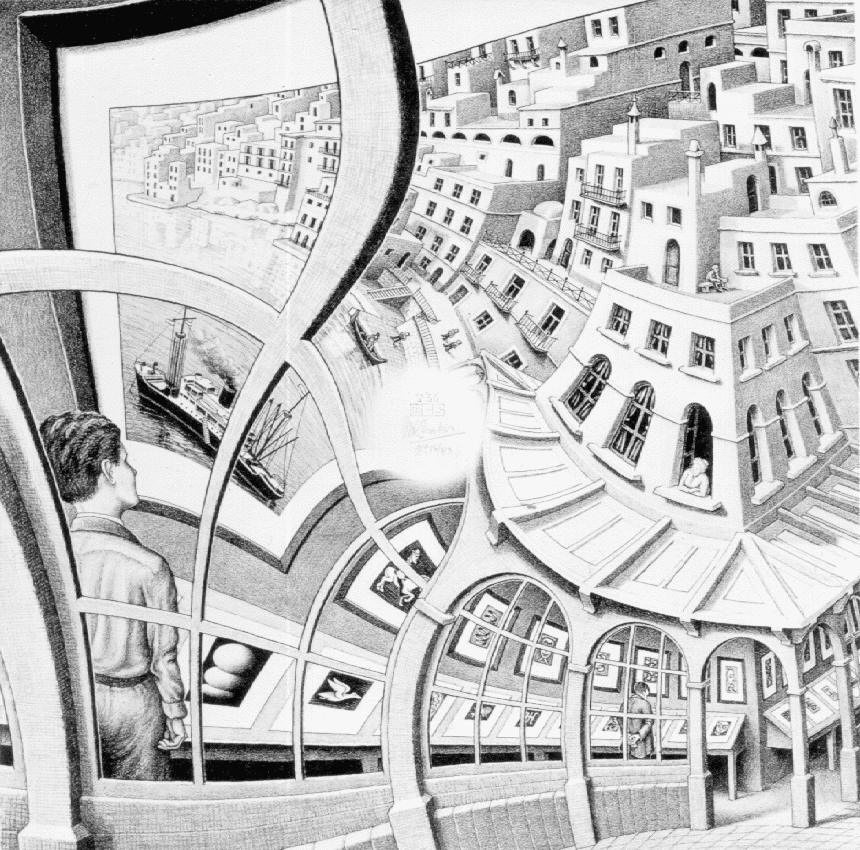
\includegraphics[width=0.5\columnwidth]{GalleriaStampe}
% The text in the square bracket is the caption for the list of figures while the text in the curly brackets is the figure caption
\caption[An example of a floating figure]{
  An example of a floating figure (a reproduction from the
  \emph{Gallery of prints}, M.~Escher,\index{Escher, M.~C.}
  from \url{http://www.mcescher.com/}).
}
\label{fig:gallery}
\end{figure}

Reference the figure composed of multiple subfigures as \autoref{fig:esempio}.
For sub-figures, reference as \autoref{fig:ipsum}.
You can also reference as \figureautorefname~\vref{fig:ipsum},
which will also add the page number where appropriate.

\lipsum[5-8] % Dummy text

\begin{figure}[tb]
\centering
\subfloat[A city market.]{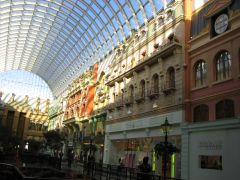
\includegraphics[width=.45\columnwidth]{Lorem}} \quad
\subfloat[Forest landscape.]{
\includegraphics[width=.45\columnwidth]{Ipsum}\label{fig:ipsum}} \\
\subfloat[Mountain landscape.]{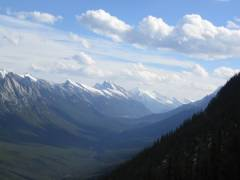
\includegraphics[width=.45\columnwidth]{Dolor}} \quad
\subfloat[A tile decoration.]{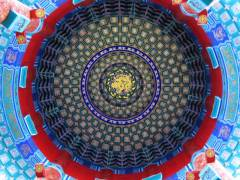
\includegraphics[width=.45\columnwidth]{Sit}}
\caption[A number of pictures.]{A number of pictures with no common theme.} % The text in the square bracket is the caption for the list of figures while the text in the curly brackets is the figure caption
\label{fig:esempio}
\end{figure}

\subsection{Comments and to-do's}
There are many ways to add to-do items.
You can use \TODO{XX}{number here} to put a note with a side-note comment.

To add a reminder to add a reference to a future section use
\todoref{Section on benefits}.

The \texttt{todonotes} package has many ways of adding to-do's.
For example, you can use \todo{Simple to-do}, or a fancy one \todo[fancyline]{Fancy!}.
You can even add \todo[inline]{an inline} todo.

\begin{comment}
Everything inside this section will be ignore.
The comment package can also support generic comment environment, and conditional comments.
\end{comment}

You can also include end notes. \endnote{example endnote}
But, this may interfere with footnotes.\footnote{a footnote}

\subsection{Math}

Some mathematics in the text: $\cos\pi=-1$ and $\alpha$.

\begin{equation}
\cos^3 \theta =\frac{1}{4}\cos\theta+\frac{3}{4}\cos 3\theta
\label{eq:refname2}
\end{equation}

\lipsum[5] % Dummy text

\begin{definition}[Gauss]
To a mathematician it is obvious that
$\int_{-\infty}^{+\infty}
e^{-x^2}\,dx=\sqrt{\pi}$.
\end{definition}

\begin{theorem}[Pythagoras]
The square of the hypotenuse (the side opposite the right angle) is equal to the sum of the squares of the other two sides.
\end{theorem}

\begin{proof}
We have that $\log(1)^2 = 2\log(1)$.
But we also have that $\log(-1)^2=\log(1)=0$.
Then $2\log(-1)=0$, from which the proof.
\end{proof}

\subsection{Methods}

\lipsum[5] % Dummy text

\begin{enumerate}[noitemsep] % [noitemsep] removes whitespace between the items for a compact look
\item First item in a list
\item Second item in a list
\item Third item in a list
\end{enumerate}

%------------------------------------------------

\subsection{Subsection}

\lipsum[11] % Dummy text

\subsubsection{Subsubsection}

\lipsum[12] % Dummy text

\begin{description}
\item[Word] Definition
\item[Concept] Explanation
\item[Idea] Text
\end{description}

\lipsum[12] % Dummy text

\begin{itemize}[noitemsep] % [noitemsep] removes whitespace between the items for a compact look
\item First item in a list
\item Second item in a list
\item Third item in a list
\end{itemize}

\subsubsection{Table}

\lipsum[13] % Dummy text

\begin{table}[hbt]
\caption{Table of Grades}
\centering
\begin{tabular}{llr}
\toprule
\multicolumn{2}{c}{Name} \\
\cmidrule(r){1-2}
First name & Last Name & Grade \\
\midrule
John & Doe & $7.5$ \\
Richard & Miles & $2$ \\
\bottomrule
\end{tabular}
\label{tab:label}
\end{table}

Reference to Table~\vref{tab:label}. % The \vref command specifies the location of the reference




%%% Local Variables:
%%% mode: latex
%%% TeX-master: "{{cookiecutter.file_name}}"
%%% End:


\section{Conclusions}
\label{sec:summary}
\lipsum[1-3]

%%% Local Variables:
%%% mode: latex
%%% TeX-master: "{{cookiecutter.file_name}}"
%%% End:

%----------------------------------------------------------------------------------------
%	BIBLIOGRAPHY
%----------------------------------------------------------------------------------------

\renewcommand{\refname}{\spacedlowsmallcaps{References}} % For modifying the bibliography heading
\printbibliography[heading=none]

\end{document}

%%% Local Variables:
%%% mode: latex
%%% TeX-master: t
%%% End:
